
% Default to the notebook output style

    


% Inherit from the specified cell style.




    
\documentclass[11pt]{article}

    
    
    \usepackage[T1]{fontenc}
    % Nicer default font (+ math font) than Computer Modern for most use cases
    \usepackage{mathpazo}
    \usepackage{float}

    % Basic figure setup, for now with no caption control since it's done
    % automatically by Pandoc (which extracts ![](path) syntax from Markdown).
    \usepackage{graphicx}
    % We will generate all images so they have a width \maxwidth. This means
    % that they will get their normal width if they fit onto the page, but
    % are scaled down if they would overflow the margins.
    \makeatletter
    \def\maxwidth{\ifdim\Gin@nat@width>\linewidth\linewidth
    \else\Gin@nat@width\fi}
    \makeatother
    \let\Oldincludegraphics\includegraphics
    % Set max figure width to be 80% of text width, for now hardcoded.
    \renewcommand{\includegraphics}[1]{\Oldincludegraphics[width=.8\maxwidth]{#1}}
    % Ensure that by default, figures have no caption (until we provide a
    % proper Figure object with a Caption API and a way to capture that
    % in the conversion process - todo).
    \usepackage{caption}
    \DeclareCaptionLabelFormat{nolabel}{}
    \captionsetup{labelformat=nolabel}

    \usepackage{adjustbox} % Used to constrain images to a maximum size 
    \usepackage{xcolor} % Allow colors to be defined
    \usepackage{enumerate} % Needed for markdown enumerations to work
    \usepackage{geometry} % Used to adjust the document margins
    \usepackage{amsmath} % Equations
    \usepackage{amssymb} % Equations
    \usepackage{textcomp} % defines textquotesingle
    % Hack from http://tex.stackexchange.com/a/47451/13684:
    \AtBeginDocument{%
        \def\PYZsq{\textquotesingle}% Upright quotes in Pygmentized code
    }
    \usepackage{upquote} % Upright quotes for verbatim code
    \usepackage{eurosym} % defines \euro
    \usepackage[mathletters]{ucs} % Extended unicode (utf-8) support
    \usepackage[utf8x]{inputenc} % Allow utf-8 characters in the tex document
    \usepackage{fancyvrb} % verbatim replacement that allows latex
    \usepackage{grffile} % extends the file name processing of package graphics 
                         % to support a larger range 
    % The hyperref package gives us a pdf with properly built
    % internal navigation ('pdf bookmarks' for the table of contents,
    % internal cross-reference links, web links for URLs, etc.)
    \usepackage{hyperref}
    \usepackage{longtable} % longtable support required by pandoc >1.10
    \usepackage{booktabs}  % table support for pandoc > 1.12.2
    \usepackage[inline]{enumitem} % IRkernel/repr support (it uses the enumerate* environment)
    \usepackage[normalem]{ulem} % ulem is needed to support strikethroughs (\sout)
                                % normalem makes italics be italics, not underlines
    \usepackage{mathrsfs}
    

    
    
    % Colors for the hyperref package
    \definecolor{urlcolor}{rgb}{0,.145,.698}
    \definecolor{linkcolor}{rgb}{.71,0.21,0.01}
    \definecolor{citecolor}{rgb}{.12,.54,.11}

    % ANSI colors
    \definecolor{ansi-black}{HTML}{3E424D}
    \definecolor{ansi-black-intense}{HTML}{282C36}
    \definecolor{ansi-red}{HTML}{E75C58}
    \definecolor{ansi-red-intense}{HTML}{B22B31}
    \definecolor{ansi-green}{HTML}{00A250}
    \definecolor{ansi-green-intense}{HTML}{007427}
    \definecolor{ansi-yellow}{HTML}{DDB62B}
    \definecolor{ansi-yellow-intense}{HTML}{B27D12}
    \definecolor{ansi-blue}{HTML}{208FFB}
    \definecolor{ansi-blue-intense}{HTML}{0065CA}
    \definecolor{ansi-magenta}{HTML}{D160C4}
    \definecolor{ansi-magenta-intense}{HTML}{A03196}
    \definecolor{ansi-cyan}{HTML}{60C6C8}
    \definecolor{ansi-cyan-intense}{HTML}{258F8F}
    \definecolor{ansi-white}{HTML}{C5C1B4}
    \definecolor{ansi-white-intense}{HTML}{A1A6B2}
    \definecolor{ansi-default-inverse-fg}{HTML}{FFFFFF}
    \definecolor{ansi-default-inverse-bg}{HTML}{000000}

    % commands and environments needed by pandoc snippets
    % extracted from the output of `pandoc -s`
    \providecommand{\tightlist}{%
      \setlength{\itemsep}{0pt}\setlength{\parskip}{0pt}}
    \DefineVerbatimEnvironment{Highlighting}{Verbatim}{commandchars=\\\{\}}
    % Add ',fontsize=\small' for more characters per line
    \newenvironment{Shaded}{}{}
    \newcommand{\KeywordTok}[1]{\textcolor[rgb]{0.00,0.44,0.13}{\textbf{{#1}}}}
    \newcommand{\DataTypeTok}[1]{\textcolor[rgb]{0.56,0.13,0.00}{{#1}}}
    \newcommand{\DecValTok}[1]{\textcolor[rgb]{0.25,0.63,0.44}{{#1}}}
    \newcommand{\BaseNTok}[1]{\textcolor[rgb]{0.25,0.63,0.44}{{#1}}}
    \newcommand{\FloatTok}[1]{\textcolor[rgb]{0.25,0.63,0.44}{{#1}}}
    \newcommand{\CharTok}[1]{\textcolor[rgb]{0.25,0.44,0.63}{{#1}}}
    \newcommand{\StringTok}[1]{\textcolor[rgb]{0.25,0.44,0.63}{{#1}}}
    \newcommand{\CommentTok}[1]{\textcolor[rgb]{0.38,0.63,0.69}{\textit{{#1}}}}
    \newcommand{\OtherTok}[1]{\textcolor[rgb]{0.00,0.44,0.13}{{#1}}}
    \newcommand{\AlertTok}[1]{\textcolor[rgb]{1.00,0.00,0.00}{\textbf{{#1}}}}
    \newcommand{\FunctionTok}[1]{\textcolor[rgb]{0.02,0.16,0.49}{{#1}}}
    \newcommand{\RegionMarkerTok}[1]{{#1}}
    \newcommand{\ErrorTok}[1]{\textcolor[rgb]{1.00,0.00,0.00}{\textbf{{#1}}}}
    \newcommand{\NormalTok}[1]{{#1}}
    
    % Additional commands for more recent versions of Pandoc
    \newcommand{\ConstantTok}[1]{\textcolor[rgb]{0.53,0.00,0.00}{{#1}}}
    \newcommand{\SpecialCharTok}[1]{\textcolor[rgb]{0.25,0.44,0.63}{{#1}}}
    \newcommand{\VerbatimStringTok}[1]{\textcolor[rgb]{0.25,0.44,0.63}{{#1}}}
    \newcommand{\SpecialStringTok}[1]{\textcolor[rgb]{0.73,0.40,0.53}{{#1}}}
    \newcommand{\ImportTok}[1]{{#1}}
    \newcommand{\DocumentationTok}[1]{\textcolor[rgb]{0.73,0.13,0.13}{\textit{{#1}}}}
    \newcommand{\AnnotationTok}[1]{\textcolor[rgb]{0.38,0.63,0.69}{\textbf{\textit{{#1}}}}}
    \newcommand{\CommentVarTok}[1]{\textcolor[rgb]{0.38,0.63,0.69}{\textbf{\textit{{#1}}}}}
    \newcommand{\VariableTok}[1]{\textcolor[rgb]{0.10,0.09,0.49}{{#1}}}
    \newcommand{\ControlFlowTok}[1]{\textcolor[rgb]{0.00,0.44,0.13}{\textbf{{#1}}}}
    \newcommand{\OperatorTok}[1]{\textcolor[rgb]{0.40,0.40,0.40}{{#1}}}
    \newcommand{\BuiltInTok}[1]{{#1}}
    \newcommand{\ExtensionTok}[1]{{#1}}
    \newcommand{\PreprocessorTok}[1]{\textcolor[rgb]{0.74,0.48,0.00}{{#1}}}
    \newcommand{\AttributeTok}[1]{\textcolor[rgb]{0.49,0.56,0.16}{{#1}}}
    \newcommand{\InformationTok}[1]{\textcolor[rgb]{0.38,0.63,0.69}{\textbf{\textit{{#1}}}}}
    \newcommand{\WarningTok}[1]{\textcolor[rgb]{0.38,0.63,0.69}{\textbf{\textit{{#1}}}}}
    
    
    % Define a nice break command that doesn't care if a line doesn't already
    % exist.
    \def\br{\hspace*{\fill} \\* }
    % Math Jax compatibility definitions
    \def\gt{>}
    \def\lt{<}
    \let\Oldtex\TeX
    \let\Oldlatex\LaTeX
    \renewcommand{\TeX}{\textrm{\Oldtex}}
    \renewcommand{\LaTeX}{\textrm{\Oldlatex}}
    % Document parameters
    % Document title
    \title{Assignment 7}
    
    \author{Jiarong Ye}
    
    
    

    % Pygments definitions
    
\makeatletter
\def\PY@reset{\let\PY@it=\relax \let\PY@bf=\relax%
    \let\PY@ul=\relax \let\PY@tc=\relax%
    \let\PY@bc=\relax \let\PY@ff=\relax}
\def\PY@tok#1{\csname PY@tok@#1\endcsname}
\def\PY@toks#1+{\ifx\relax#1\empty\else%
    \PY@tok{#1}\expandafter\PY@toks\fi}
\def\PY@do#1{\PY@bc{\PY@tc{\PY@ul{%
    \PY@it{\PY@bf{\PY@ff{#1}}}}}}}
\def\PY#1#2{\PY@reset\PY@toks#1+\relax+\PY@do{#2}}

\expandafter\def\csname PY@tok@w\endcsname{\def\PY@tc##1{\textcolor[rgb]{0.73,0.73,0.73}{##1}}}
\expandafter\def\csname PY@tok@c\endcsname{\let\PY@it=\textit\def\PY@tc##1{\textcolor[rgb]{0.25,0.50,0.50}{##1}}}
\expandafter\def\csname PY@tok@cp\endcsname{\def\PY@tc##1{\textcolor[rgb]{0.74,0.48,0.00}{##1}}}
\expandafter\def\csname PY@tok@k\endcsname{\let\PY@bf=\textbf\def\PY@tc##1{\textcolor[rgb]{0.00,0.50,0.00}{##1}}}
\expandafter\def\csname PY@tok@kp\endcsname{\def\PY@tc##1{\textcolor[rgb]{0.00,0.50,0.00}{##1}}}
\expandafter\def\csname PY@tok@kt\endcsname{\def\PY@tc##1{\textcolor[rgb]{0.69,0.00,0.25}{##1}}}
\expandafter\def\csname PY@tok@o\endcsname{\def\PY@tc##1{\textcolor[rgb]{0.40,0.40,0.40}{##1}}}
\expandafter\def\csname PY@tok@ow\endcsname{\let\PY@bf=\textbf\def\PY@tc##1{\textcolor[rgb]{0.67,0.13,1.00}{##1}}}
\expandafter\def\csname PY@tok@nb\endcsname{\def\PY@tc##1{\textcolor[rgb]{0.00,0.50,0.00}{##1}}}
\expandafter\def\csname PY@tok@nf\endcsname{\def\PY@tc##1{\textcolor[rgb]{0.00,0.00,1.00}{##1}}}
\expandafter\def\csname PY@tok@nc\endcsname{\let\PY@bf=\textbf\def\PY@tc##1{\textcolor[rgb]{0.00,0.00,1.00}{##1}}}
\expandafter\def\csname PY@tok@nn\endcsname{\let\PY@bf=\textbf\def\PY@tc##1{\textcolor[rgb]{0.00,0.00,1.00}{##1}}}
\expandafter\def\csname PY@tok@ne\endcsname{\let\PY@bf=\textbf\def\PY@tc##1{\textcolor[rgb]{0.82,0.25,0.23}{##1}}}
\expandafter\def\csname PY@tok@nv\endcsname{\def\PY@tc##1{\textcolor[rgb]{0.10,0.09,0.49}{##1}}}
\expandafter\def\csname PY@tok@no\endcsname{\def\PY@tc##1{\textcolor[rgb]{0.53,0.00,0.00}{##1}}}
\expandafter\def\csname PY@tok@nl\endcsname{\def\PY@tc##1{\textcolor[rgb]{0.63,0.63,0.00}{##1}}}
\expandafter\def\csname PY@tok@ni\endcsname{\let\PY@bf=\textbf\def\PY@tc##1{\textcolor[rgb]{0.60,0.60,0.60}{##1}}}
\expandafter\def\csname PY@tok@na\endcsname{\def\PY@tc##1{\textcolor[rgb]{0.49,0.56,0.16}{##1}}}
\expandafter\def\csname PY@tok@nt\endcsname{\let\PY@bf=\textbf\def\PY@tc##1{\textcolor[rgb]{0.00,0.50,0.00}{##1}}}
\expandafter\def\csname PY@tok@nd\endcsname{\def\PY@tc##1{\textcolor[rgb]{0.67,0.13,1.00}{##1}}}
\expandafter\def\csname PY@tok@s\endcsname{\def\PY@tc##1{\textcolor[rgb]{0.73,0.13,0.13}{##1}}}
\expandafter\def\csname PY@tok@sd\endcsname{\let\PY@it=\textit\def\PY@tc##1{\textcolor[rgb]{0.73,0.13,0.13}{##1}}}
\expandafter\def\csname PY@tok@si\endcsname{\let\PY@bf=\textbf\def\PY@tc##1{\textcolor[rgb]{0.73,0.40,0.53}{##1}}}
\expandafter\def\csname PY@tok@se\endcsname{\let\PY@bf=\textbf\def\PY@tc##1{\textcolor[rgb]{0.73,0.40,0.13}{##1}}}
\expandafter\def\csname PY@tok@sr\endcsname{\def\PY@tc##1{\textcolor[rgb]{0.73,0.40,0.53}{##1}}}
\expandafter\def\csname PY@tok@ss\endcsname{\def\PY@tc##1{\textcolor[rgb]{0.10,0.09,0.49}{##1}}}
\expandafter\def\csname PY@tok@sx\endcsname{\def\PY@tc##1{\textcolor[rgb]{0.00,0.50,0.00}{##1}}}
\expandafter\def\csname PY@tok@m\endcsname{\def\PY@tc##1{\textcolor[rgb]{0.40,0.40,0.40}{##1}}}
\expandafter\def\csname PY@tok@gh\endcsname{\let\PY@bf=\textbf\def\PY@tc##1{\textcolor[rgb]{0.00,0.00,0.50}{##1}}}
\expandafter\def\csname PY@tok@gu\endcsname{\let\PY@bf=\textbf\def\PY@tc##1{\textcolor[rgb]{0.50,0.00,0.50}{##1}}}
\expandafter\def\csname PY@tok@gd\endcsname{\def\PY@tc##1{\textcolor[rgb]{0.63,0.00,0.00}{##1}}}
\expandafter\def\csname PY@tok@gi\endcsname{\def\PY@tc##1{\textcolor[rgb]{0.00,0.63,0.00}{##1}}}
\expandafter\def\csname PY@tok@gr\endcsname{\def\PY@tc##1{\textcolor[rgb]{1.00,0.00,0.00}{##1}}}
\expandafter\def\csname PY@tok@ge\endcsname{\let\PY@it=\textit}
\expandafter\def\csname PY@tok@gs\endcsname{\let\PY@bf=\textbf}
\expandafter\def\csname PY@tok@gp\endcsname{\let\PY@bf=\textbf\def\PY@tc##1{\textcolor[rgb]{0.00,0.00,0.50}{##1}}}
\expandafter\def\csname PY@tok@go\endcsname{\def\PY@tc##1{\textcolor[rgb]{0.53,0.53,0.53}{##1}}}
\expandafter\def\csname PY@tok@gt\endcsname{\def\PY@tc##1{\textcolor[rgb]{0.00,0.27,0.87}{##1}}}
\expandafter\def\csname PY@tok@err\endcsname{\def\PY@bc##1{\setlength{\fboxsep}{0pt}\fcolorbox[rgb]{1.00,0.00,0.00}{1,1,1}{\strut ##1}}}
\expandafter\def\csname PY@tok@kc\endcsname{\let\PY@bf=\textbf\def\PY@tc##1{\textcolor[rgb]{0.00,0.50,0.00}{##1}}}
\expandafter\def\csname PY@tok@kd\endcsname{\let\PY@bf=\textbf\def\PY@tc##1{\textcolor[rgb]{0.00,0.50,0.00}{##1}}}
\expandafter\def\csname PY@tok@kn\endcsname{\let\PY@bf=\textbf\def\PY@tc##1{\textcolor[rgb]{0.00,0.50,0.00}{##1}}}
\expandafter\def\csname PY@tok@kr\endcsname{\let\PY@bf=\textbf\def\PY@tc##1{\textcolor[rgb]{0.00,0.50,0.00}{##1}}}
\expandafter\def\csname PY@tok@bp\endcsname{\def\PY@tc##1{\textcolor[rgb]{0.00,0.50,0.00}{##1}}}
\expandafter\def\csname PY@tok@fm\endcsname{\def\PY@tc##1{\textcolor[rgb]{0.00,0.00,1.00}{##1}}}
\expandafter\def\csname PY@tok@vc\endcsname{\def\PY@tc##1{\textcolor[rgb]{0.10,0.09,0.49}{##1}}}
\expandafter\def\csname PY@tok@vg\endcsname{\def\PY@tc##1{\textcolor[rgb]{0.10,0.09,0.49}{##1}}}
\expandafter\def\csname PY@tok@vi\endcsname{\def\PY@tc##1{\textcolor[rgb]{0.10,0.09,0.49}{##1}}}
\expandafter\def\csname PY@tok@vm\endcsname{\def\PY@tc##1{\textcolor[rgb]{0.10,0.09,0.49}{##1}}}
\expandafter\def\csname PY@tok@sa\endcsname{\def\PY@tc##1{\textcolor[rgb]{0.73,0.13,0.13}{##1}}}
\expandafter\def\csname PY@tok@sb\endcsname{\def\PY@tc##1{\textcolor[rgb]{0.73,0.13,0.13}{##1}}}
\expandafter\def\csname PY@tok@sc\endcsname{\def\PY@tc##1{\textcolor[rgb]{0.73,0.13,0.13}{##1}}}
\expandafter\def\csname PY@tok@dl\endcsname{\def\PY@tc##1{\textcolor[rgb]{0.73,0.13,0.13}{##1}}}
\expandafter\def\csname PY@tok@s2\endcsname{\def\PY@tc##1{\textcolor[rgb]{0.73,0.13,0.13}{##1}}}
\expandafter\def\csname PY@tok@sh\endcsname{\def\PY@tc##1{\textcolor[rgb]{0.73,0.13,0.13}{##1}}}
\expandafter\def\csname PY@tok@s1\endcsname{\def\PY@tc##1{\textcolor[rgb]{0.73,0.13,0.13}{##1}}}
\expandafter\def\csname PY@tok@mb\endcsname{\def\PY@tc##1{\textcolor[rgb]{0.40,0.40,0.40}{##1}}}
\expandafter\def\csname PY@tok@mf\endcsname{\def\PY@tc##1{\textcolor[rgb]{0.40,0.40,0.40}{##1}}}
\expandafter\def\csname PY@tok@mh\endcsname{\def\PY@tc##1{\textcolor[rgb]{0.40,0.40,0.40}{##1}}}
\expandafter\def\csname PY@tok@mi\endcsname{\def\PY@tc##1{\textcolor[rgb]{0.40,0.40,0.40}{##1}}}
\expandafter\def\csname PY@tok@il\endcsname{\def\PY@tc##1{\textcolor[rgb]{0.40,0.40,0.40}{##1}}}
\expandafter\def\csname PY@tok@mo\endcsname{\def\PY@tc##1{\textcolor[rgb]{0.40,0.40,0.40}{##1}}}
\expandafter\def\csname PY@tok@ch\endcsname{\let\PY@it=\textit\def\PY@tc##1{\textcolor[rgb]{0.25,0.50,0.50}{##1}}}
\expandafter\def\csname PY@tok@cm\endcsname{\let\PY@it=\textit\def\PY@tc##1{\textcolor[rgb]{0.25,0.50,0.50}{##1}}}
\expandafter\def\csname PY@tok@cpf\endcsname{\let\PY@it=\textit\def\PY@tc##1{\textcolor[rgb]{0.25,0.50,0.50}{##1}}}
\expandafter\def\csname PY@tok@c1\endcsname{\let\PY@it=\textit\def\PY@tc##1{\textcolor[rgb]{0.25,0.50,0.50}{##1}}}
\expandafter\def\csname PY@tok@cs\endcsname{\let\PY@it=\textit\def\PY@tc##1{\textcolor[rgb]{0.25,0.50,0.50}{##1}}}

\def\PYZbs{\char`\\}
\def\PYZus{\char`\_}
\def\PYZob{\char`\{}
\def\PYZcb{\char`\}}
\def\PYZca{\char`\^}
\def\PYZam{\char`\&}
\def\PYZlt{\char`\<}
\def\PYZgt{\char`\>}
\def\PYZsh{\char`\#}
\def\PYZpc{\char`\%}
\def\PYZdl{\char`\$}
\def\PYZhy{\char`\-}
\def\PYZsq{\char`\'}
\def\PYZdq{\char`\"}
\def\PYZti{\char`\~}
% for compatibility with earlier versions
\def\PYZat{@}
\def\PYZlb{[}
\def\PYZrb{]}
\makeatother


    % Exact colors from NB
    \definecolor{incolor}{rgb}{0.0, 0.0, 0.5}
    \definecolor{outcolor}{rgb}{0.545, 0.0, 0.0}



    
    % Prevent overflowing lines due to hard-to-break entities
    \sloppy 
    % Setup hyperref package
    \hypersetup{
      breaklinks=true,  % so long urls are correctly broken across lines
      colorlinks=true,
      urlcolor=urlcolor,
      linkcolor=linkcolor,
      citecolor=citecolor,
      }
    % Slightly bigger margins than the latex defaults
    
    \geometry{verbose,tmargin=1in,bmargin=1in,lmargin=1in,rmargin=1in, left=2cm, right=1cm}
    
    

    \begin{document}
    
    
    \maketitle
    
    

    
    \subsection*{Load the data}\label{load-the-data}

    \begin{Verbatim}[commandchars=\\\{\}]
{\color{incolor}In [{\color{incolor}40}]:} \PY{k+kn}{import} \PY{n+nn}{pandas} \PY{k}{as} \PY{n+nn}{pd}
         \PY{k+kn}{from} \PY{n+nn}{datetime} \PY{k}{import} \PY{n}{datetime}
         \PY{k+kn}{import} \PY{n+nn}{pymysql} 
\end{Verbatim}

    \begin{Verbatim}[commandchars=\\\{\}]
{\color{incolor}In [{\color{incolor}41}]:} \PY{n}{department} \PY{o}{=} \PY{n}{pd}\PY{o}{.}\PY{n}{read\PYZus{}csv}\PY{p}{(}\PY{l+s+s1}{\PYZsq{}}\PY{l+s+s1}{departments.csv}\PY{l+s+s1}{\PYZsq{}}\PY{p}{,} \PY{n}{sep}\PY{o}{=}\PY{l+s+s1}{\PYZsq{}}\PY{l+s+s1}{,}\PY{l+s+s1}{\PYZsq{}}\PY{p}{)}
         \PY{n}{department}\PY{o}{.}\PY{n}{columns} \PY{o}{=} \PY{p}{[}\PY{l+s+s1}{\PYZsq{}}\PY{l+s+s1}{department\PYZus{}name}\PY{l+s+s1}{\PYZsq{}}\PY{p}{]}
         \PY{n}{shift} \PY{o}{=} \PY{n}{pd}\PY{o}{.}\PY{n}{read\PYZus{}csv}\PY{p}{(}\PY{l+s+s1}{\PYZsq{}}\PY{l+s+s1}{shifts.csv}\PY{l+s+s1}{\PYZsq{}}\PY{p}{,} \PY{n}{sep}\PY{o}{=}\PY{l+s+s1}{\PYZsq{}}\PY{l+s+s1}{,}\PY{l+s+s1}{\PYZsq{}}\PY{p}{)}
         \PY{n}{shift}\PY{o}{.}\PY{n}{columns} \PY{o}{=} \PY{p}{[}\PY{l+s+s1}{\PYZsq{}}\PY{l+s+s1}{from\PYZus{}time}\PY{l+s+s1}{\PYZsq{}}\PY{p}{,} \PY{l+s+s1}{\PYZsq{}}\PY{l+s+s1}{length}\PY{l+s+s1}{\PYZsq{}}\PY{p}{]}
         \PY{n}{employees} \PY{o}{=} \PY{n}{pd}\PY{o}{.}\PY{n}{read\PYZus{}csv}\PY{p}{(}\PY{l+s+s1}{\PYZsq{}}\PY{l+s+s1}{employees.csv}\PY{l+s+s1}{\PYZsq{}}\PY{p}{,} \PY{n}{sep}\PY{o}{=}\PY{l+s+s1}{\PYZsq{}}\PY{l+s+s1}{,}\PY{l+s+s1}{\PYZsq{}}\PY{p}{)}
         \PY{n}{employees}\PY{o}{.}\PY{n}{emptype} \PY{o}{=} \PY{n}{employees}\PY{o}{.}\PY{n}{emptype}\PY{o}{.}\PY{n}{fillna}\PY{p}{(}\PY{l+s+s1}{\PYZsq{}}\PY{l+s+s1}{\PYZsq{}}\PY{p}{)}
         \PY{n}{schedule} \PY{o}{=} \PY{n}{pd}\PY{o}{.}\PY{n}{read\PYZus{}csv}\PY{p}{(}\PY{l+s+s1}{\PYZsq{}}\PY{l+s+s1}{schedule.csv}\PY{l+s+s1}{\PYZsq{}}\PY{p}{,} \PY{n}{sep}\PY{o}{=}\PY{l+s+s1}{\PYZsq{}}\PY{l+s+s1}{,}\PY{l+s+s1}{\PYZsq{}}\PY{p}{)}
         \PY{n}{schedule}\PY{o}{.}\PY{n}{columns} \PY{o}{=} \PY{p}{[}\PY{l+s+s1}{\PYZsq{}}\PY{l+s+s1}{date}\PY{l+s+s1}{\PYZsq{}}\PY{p}{,} \PY{l+s+s1}{\PYZsq{}}\PY{l+s+s1}{empid}\PY{l+s+s1}{\PYZsq{}}\PY{p}{,} \PY{l+s+s1}{\PYZsq{}}\PY{l+s+s1}{dept}\PY{l+s+s1}{\PYZsq{}}\PY{p}{,} \PY{l+s+s1}{\PYZsq{}}\PY{l+s+s1}{start\PYZus{}time}\PY{l+s+s1}{\PYZsq{}}\PY{p}{,} \PY{l+s+s1}{\PYZsq{}}\PY{l+s+s1}{shift\PYZus{}length}\PY{l+s+s1}{\PYZsq{}}\PY{p}{]}
\end{Verbatim}

    \subsection*{Manipulate the data}\label{manipulate-the-data}

    \begin{Verbatim}[commandchars=\\\{\}]
{\color{incolor}In [{\color{incolor}48}]:} \PY{k}{class} \PY{n+nc}{DataSqlLoader}\PY{p}{:}
             \PY{k}{def} \PY{n+nf}{\PYZus{}\PYZus{}init\PYZus{}\PYZus{}}\PY{p}{(}\PY{n+nb+bp}{self}\PY{p}{,} \PY{n}{database}\PY{p}{)}\PY{p}{:}
                 \PY{c+c1}{\PYZsh{} connect to mysql local server}
                 \PY{n+nb+bp}{self}\PY{o}{.}\PY{n}{db} \PY{o}{=} \PY{n}{pymysql}\PY{o}{.}\PY{n}{Connect}\PY{p}{(}
                     \PY{n}{host}\PY{o}{=}\PY{l+s+s1}{\PYZsq{}}\PY{l+s+s1}{us\PYZhy{}cdbr\PYZhy{}iron\PYZhy{}east\PYZhy{}01.cleardb.net}\PY{l+s+s1}{\PYZsq{}}\PY{p}{,} 
                     \PY{n}{port}\PY{o}{=}\PY{l+m+mi}{3306}\PY{p}{,} 
                     \PY{n}{user}\PY{o}{=}\PY{l+s+s1}{\PYZsq{}}\PY{l+s+s1}{b033ff6b193dc0}\PY{l+s+s1}{\PYZsq{}}\PY{p}{,} 
                     \PY{n}{passwd}\PY{o}{=}\PY{l+s+s1}{\PYZsq{}}\PY{l+s+s1}{02f96442}\PY{l+s+s1}{\PYZsq{}}\PY{p}{,} 
                     \PY{n}{db}\PY{o}{=}\PY{n}{database}\PY{p}{)}
                 \PY{n+nb+bp}{self}\PY{o}{.}\PY{n}{c} \PY{o}{=} \PY{n+nb+bp}{self}\PY{o}{.}\PY{n}{db}\PY{o}{.}\PY{n}{cursor}\PY{p}{(}\PY{p}{)}
             
             \PY{c+c1}{\PYZsh{} convert the shift and schedule time to `time` format compatible in MySQL}
             \PY{k}{def} \PY{n+nf}{convert\PYZus{}time\PYZus{}format}\PY{p}{(}\PY{n+nb+bp}{self}\PY{p}{,} \PY{n}{time}\PY{p}{)}\PY{p}{:}
                 \PY{k}{return} \PY{n}{datetime}\PY{o}{.}\PY{n}{strptime}\PY{p}{(}\PY{l+s+s1}{\PYZsq{}}\PY{l+s+si}{\PYZob{}\PYZcb{}}\PY{l+s+s1}{\PYZsq{}}\PY{o}{.}\PY{n}{format}\PY{p}{(}\PY{n}{time}\PY{p}{)}\PY{p}{,} \PY{l+s+s1}{\PYZsq{}}\PY{l+s+s1}{\PYZpc{}}\PY{l+s+s1}{I}\PY{l+s+s1}{\PYZpc{}}\PY{l+s+s1}{p}\PY{l+s+s1}{\PYZsq{}}\PY{p}{)}\PY{o}{.}\PY{n}{strftime}\PY{p}{(}\PY{l+s+s1}{\PYZsq{}}\PY{l+s+s1}{\PYZpc{}}\PY{l+s+s1}{H:}\PY{l+s+s1}{\PYZpc{}}\PY{l+s+s1}{M:}\PY{l+s+s1}{\PYZpc{}}\PY{l+s+s1}{S}\PY{l+s+s1}{\PYZsq{}}\PY{p}{)}
             
             \PY{c+c1}{\PYZsh{} convert schedule date to `date` format compatible in MySQL}
             \PY{k}{def} \PY{n+nf}{convert\PYZus{}date\PYZus{}format}\PY{p}{(}\PY{n+nb+bp}{self}\PY{p}{,} \PY{n}{time}\PY{p}{)}\PY{p}{:}
                 \PY{k}{return} \PY{n}{datetime}\PY{o}{.}\PY{n}{strptime}\PY{p}{(}\PY{l+s+s1}{\PYZsq{}}\PY{l+s+si}{\PYZob{}\PYZcb{}}\PY{l+s+s1}{\PYZsq{}}\PY{o}{.}\PY{n}{format}\PY{p}{(}\PY{n}{time}\PY{p}{)}\PY{p}{,} \PY{l+s+s1}{\PYZsq{}}\PY{l+s+s1}{\PYZpc{}}\PY{l+s+s1}{m/}\PY{l+s+si}{\PYZpc{}d}\PY{l+s+s1}{/}\PY{l+s+s1}{\PYZpc{}}\PY{l+s+s1}{Y}\PY{l+s+s1}{\PYZsq{}}\PY{p}{)}\PY{o}{.}\PY{n}{strftime}\PY{p}{(}\PY{l+s+s1}{\PYZsq{}}\PY{l+s+s1}{\PYZpc{}}\PY{l+s+s1}{Y\PYZhy{}}\PY{l+s+s1}{\PYZpc{}}\PY{l+s+s1}{m\PYZhy{}}\PY{l+s+si}{\PYZpc{}d}\PY{l+s+s1}{\PYZsq{}}\PY{p}{)}
             
             \PY{k}{def} \PY{n+nf}{creat\PYZus{}tables}\PY{p}{(}\PY{n+nb+bp}{self}\PY{p}{)}\PY{p}{:}
                 \PY{n+nb+bp}{self}\PY{o}{.}\PY{n}{c}\PY{o}{.}\PY{n}{execute}\PY{p}{(}\PY{l+s+s1}{\PYZsq{}\PYZsq{}\PYZsq{}}
         \PY{l+s+s1}{                create table if not exists department}
         \PY{l+s+s1}{                (}
         \PY{l+s+s1}{                  department\PYZus{}id  int auto\PYZus{}increment}
         \PY{l+s+s1}{                    primary key,}
         \PY{l+s+s1}{                  department\PYZus{}name varchar(50) not null}
         \PY{l+s+s1}{                );}
         \PY{l+s+s1}{                }\PY{l+s+s1}{\PYZsq{}\PYZsq{}\PYZsq{}}\PY{p}{)}
                 \PY{n+nb+bp}{self}\PY{o}{.}\PY{n}{c}\PY{o}{.}\PY{n}{execute}\PY{p}{(}\PY{l+s+s1}{\PYZsq{}\PYZsq{}\PYZsq{}}
         \PY{l+s+s1}{            create table if not exists shift}
         \PY{l+s+s1}{            (}
         \PY{l+s+s1}{              shift\PYZus{}id int auto\PYZus{}increment}
         \PY{l+s+s1}{                primary key,}
         \PY{l+s+s1}{              from\PYZus{}time   time not null,}
         \PY{l+s+s1}{              length   int  not null}
         \PY{l+s+s1}{            );}
         \PY{l+s+s1}{            }\PY{l+s+s1}{\PYZsq{}\PYZsq{}\PYZsq{}}\PY{p}{)}
                 \PY{n+nb+bp}{self}\PY{o}{.}\PY{n}{c}\PY{o}{.}\PY{n}{execute}\PY{p}{(}\PY{l+s+s1}{\PYZsq{}\PYZsq{}\PYZsq{}}
         \PY{l+s+s1}{            create table if not exists schedule}
         \PY{l+s+s1}{            (}
         \PY{l+s+s1}{              schedule\PYZus{}id  int auto\PYZus{}increment}
         \PY{l+s+s1}{                primary key,}
         \PY{l+s+s1}{              date         date        not null,}
         \PY{l+s+s1}{              empid        varchar(10) not null,}
         \PY{l+s+s1}{              dept         varchar(50) not null,}
         \PY{l+s+s1}{              start\PYZus{}time   time        not null,}
         \PY{l+s+s1}{              shift\PYZus{}length int         not null}
         \PY{l+s+s1}{            );}
         \PY{l+s+s1}{            }\PY{l+s+s1}{\PYZsq{}\PYZsq{}\PYZsq{}}\PY{p}{)}
                 \PY{n+nb+bp}{self}\PY{o}{.}\PY{n}{c}\PY{o}{.}\PY{n}{execute}\PY{p}{(}\PY{l+s+s1}{\PYZsq{}\PYZsq{}\PYZsq{}}
         \PY{l+s+s1}{            create table if not exists employees}
         \PY{l+s+s1}{            (}
         \PY{l+s+s1}{              empid     varchar(10) not null primary key,}
         \PY{l+s+s1}{              lastname  varchar(20) not null,}
         \PY{l+s+s1}{              firstname varchar(20) not null,}
         \PY{l+s+s1}{              emptype   varchar(3)  null,}
         \PY{l+s+s1}{              cellphone varchar(20) null,}
         \PY{l+s+s1}{              homephone varchar(20) null,}
         \PY{l+s+s1}{              ftpt      varchar(2)  not null,}
         \PY{l+s+s1}{              constraint employee\PYZus{}empid\PYZus{}uindex}
         \PY{l+s+s1}{              unique (empid)}
         \PY{l+s+s1}{            );}
         \PY{l+s+s1}{        }\PY{l+s+s1}{\PYZsq{}\PYZsq{}\PYZsq{}}\PY{p}{)}
                 
                 \PY{n+nb+bp}{self}\PY{o}{.}\PY{n}{c}\PY{o}{.}\PY{n}{execute}\PY{p}{(}\PY{l+s+s1}{\PYZsq{}\PYZsq{}\PYZsq{}}
         \PY{l+s+s1}{            create table if not exists department\PYZus{}managers}
         \PY{l+s+s1}{            (}
         \PY{l+s+s1}{                dept\PYZus{}name varchar(20),}
         \PY{l+s+s1}{                manager varchar(30)}
         \PY{l+s+s1}{            );}
         \PY{l+s+s1}{        }\PY{l+s+s1}{\PYZsq{}\PYZsq{}\PYZsq{}}\PY{p}{)}
             
             \PY{k}{def} \PY{n+nf}{insert\PYZus{}into\PYZus{}tables}\PY{p}{(}\PY{n+nb+bp}{self}\PY{p}{,} \PY{n}{table}\PY{p}{,} \PY{n}{table\PYZus{}name}\PY{p}{)}\PY{p}{:}
                 \PY{k}{for} \PY{n}{i} \PY{o+ow}{in} \PY{n+nb}{range}\PY{p}{(}\PY{n+nb}{len}\PY{p}{(}\PY{n}{table}\PY{p}{)}\PY{p}{)}\PY{p}{:}
                     \PY{n}{attributes} \PY{o}{=} \PY{l+s+s1}{\PYZsq{}}\PY{l+s+si}{\PYZob{}\PYZcb{}}\PY{l+s+s1}{\PYZsq{}}\PY{o}{.}\PY{n}{format}\PY{p}{(}\PY{n+nb}{tuple}\PY{p}{(}\PY{n}{table}\PY{o}{.}\PY{n}{columns}\PY{o}{.}\PY{n}{tolist}\PY{p}{(}\PY{p}{)}\PY{p}{)}\PY{p}{)}\PY{o}{.}\PY{n}{replace}\PY{p}{(}\PY{l+s+s2}{\PYZdq{}}\PY{l+s+s2}{\PYZsq{}}\PY{l+s+s2}{\PYZdq{}}\PY{p}{,}\PY{l+s+s2}{\PYZdq{}}\PY{l+s+s2}{\PYZdq{}}\PY{p}{)}
                     \PY{n}{query} \PY{o}{=} \PY{l+s+s2}{\PYZdq{}}\PY{l+s+s2}{insert into }\PY{l+s+si}{\PYZob{}\PYZcb{}}\PY{l+s+s2}{ }\PY{l+s+si}{\PYZob{}\PYZcb{}}\PY{l+s+s2}{ values }\PY{l+s+si}{\PYZob{}\PYZcb{}}\PY{l+s+s2}{;}\PY{l+s+s2}{\PYZdq{}}\PY{o}{.}\PY{n}{format}\PY{p}{(}
                         \PY{n}{table\PYZus{}name}\PY{p}{,} \PY{n}{attributes}\PY{p}{,} \PY{n+nb}{tuple}\PY{p}{(}\PY{n}{table}\PY{o}{.}\PY{n}{iloc}\PY{p}{[}\PY{n}{i}\PY{p}{,}\PY{p}{:}\PY{p}{]}\PY{o}{.}\PY{n}{values}\PY{p}{)}\PY{p}{)}
                     \PY{n}{query} \PY{o}{=} \PY{n}{query}\PY{o}{.}\PY{n}{replace}\PY{p}{(}\PY{l+s+s2}{\PYZdq{}}\PY{l+s+s2}{(none)}\PY{l+s+s2}{\PYZdq{}}\PY{p}{,}\PY{l+s+s2}{\PYZdq{}}\PY{l+s+s2}{\PYZdq{}}\PY{p}{)}
                     \PY{n}{query} \PY{o}{=} \PY{n}{query}\PY{o}{.}\PY{n}{replace}\PY{p}{(}\PY{l+s+sa}{r}\PY{l+s+s2}{\PYZdq{}}\PY{l+s+s2}{,)}\PY{l+s+s2}{\PYZdq{}}\PY{p}{,}\PY{l+s+s2}{\PYZdq{}}\PY{l+s+s2}{)}\PY{l+s+s2}{\PYZdq{}}\PY{p}{)}
                     \PY{c+c1}{\PYZsh{} print(query)}
                     \PY{k}{try}\PY{p}{:}
                         \PY{n+nb+bp}{self}\PY{o}{.}\PY{n}{c}\PY{o}{.}\PY{n}{execute}\PY{p}{(}\PY{n}{query}\PY{p}{)}
                         \PY{n+nb+bp}{self}\PY{o}{.}\PY{n}{db}\PY{o}{.}\PY{n}{commit}\PY{p}{(}\PY{p}{)}
                     \PY{k}{except} \PY{n+ne}{Exception} \PY{k}{as} \PY{n}{e}\PY{p}{:}
                         \PY{n+nb}{print}\PY{p}{(}\PY{n}{e}\PY{p}{)}
                         
             \PY{k}{def} \PY{n+nf}{close}\PY{p}{(}\PY{n+nb+bp}{self}\PY{p}{)}\PY{p}{:}
                 \PY{n+nb+bp}{self}\PY{o}{.}\PY{n}{db}\PY{o}{.}\PY{n}{close}\PY{p}{(}\PY{p}{)}
\end{Verbatim}

    \begin{Verbatim}[commandchars=\\\{\}]
{\color{incolor}In [{\color{incolor}110}]:} \PY{n}{dsl} \PY{o}{=} \PY{n}{DataSqlLoader}\PY{p}{(}\PY{l+s+s1}{\PYZsq{}}\PY{l+s+s1}{heroku\PYZus{}f2b490785080ebd}\PY{l+s+s1}{\PYZsq{}}\PY{p}{)}
          \PY{n}{dsl}\PY{o}{.}\PY{n}{creat\PYZus{}tables}\PY{p}{(}\PY{p}{)}
          
          \PY{n}{schedule}\PY{p}{[}\PY{l+s+s1}{\PYZsq{}}\PY{l+s+s1}{start\PYZus{}time}\PY{l+s+s1}{\PYZsq{}}\PY{p}{]} \PY{o}{=} \PY{n+nb}{list}\PY{p}{(}\PY{n+nb}{map}\PY{p}{(}\PY{k}{lambda} \PY{n}{x}\PY{p}{:} \PY{n}{dsl}\PY{o}{.}\PY{n}{convert\PYZus{}time\PYZus{}format}\PY{p}{(}\PY{n}{x}\PY{p}{)}\PY{p}{,} 
                                            \PY{n}{schedule}\PY{p}{[}\PY{l+s+s1}{\PYZsq{}}\PY{l+s+s1}{start\PYZus{}time}\PY{l+s+s1}{\PYZsq{}}\PY{p}{]}\PY{p}{)}\PY{p}{)}
          \PY{n}{shift}\PY{p}{[}\PY{l+s+s1}{\PYZsq{}}\PY{l+s+s1}{from\PYZus{}time}\PY{l+s+s1}{\PYZsq{}}\PY{p}{]} \PY{o}{=} \PY{n+nb}{list}\PY{p}{(}\PY{n+nb}{map}\PY{p}{(}\PY{k}{lambda} \PY{n}{x}\PY{p}{:} \PY{n}{dsl}\PY{o}{.}\PY{n}{convert\PYZus{}time\PYZus{}format}\PY{p}{(}\PY{n}{x}\PY{p}{)}\PY{p}{,} 
                                        \PY{n}{shift}\PY{p}{[}\PY{l+s+s1}{\PYZsq{}}\PY{l+s+s1}{from\PYZus{}time}\PY{l+s+s1}{\PYZsq{}}\PY{p}{]}\PY{p}{)}\PY{p}{)}
          \PY{n}{schedule}\PY{p}{[}\PY{l+s+s1}{\PYZsq{}}\PY{l+s+s1}{date}\PY{l+s+s1}{\PYZsq{}}\PY{p}{]} \PY{o}{=} \PY{n+nb}{list}\PY{p}{(}\PY{n+nb}{map}\PY{p}{(}\PY{k}{lambda} \PY{n}{x}\PY{p}{:} \PY{n}{dsl}\PY{o}{.}\PY{n}{convert\PYZus{}date\PYZus{}format}\PY{p}{(}\PY{n}{x}\PY{p}{)}\PY{p}{,} 
                                      \PY{n}{schedule}\PY{p}{[}\PY{l+s+s1}{\PYZsq{}}\PY{l+s+s1}{date}\PY{l+s+s1}{\PYZsq{}}\PY{p}{]}\PY{p}{)}\PY{p}{)}
          
          \PY{n}{dsl}\PY{o}{.}\PY{n}{insert\PYZus{}into\PYZus{}tables}\PY{p}{(}\PY{n}{department}\PY{p}{,} \PY{l+s+s1}{\PYZsq{}}\PY{l+s+s1}{department}\PY{l+s+s1}{\PYZsq{}}\PY{p}{)}
          \PY{n}{dsl}\PY{o}{.}\PY{n}{insert\PYZus{}into\PYZus{}tables}\PY{p}{(}\PY{n}{shift}\PY{p}{,} \PY{l+s+s1}{\PYZsq{}}\PY{l+s+s1}{shift}\PY{l+s+s1}{\PYZsq{}}\PY{p}{)}
          \PY{n}{dsl}\PY{o}{.}\PY{n}{insert\PYZus{}into\PYZus{}tables}\PY{p}{(}\PY{n}{schedule}\PY{p}{,}\PY{l+s+s1}{\PYZsq{}}\PY{l+s+s1}{schedule}\PY{l+s+s1}{\PYZsq{}}\PY{p}{)}
          \PY{n}{dsl}\PY{o}{.}\PY{n}{insert\PYZus{}into\PYZus{}tables}\PY{p}{(}\PY{n}{employees}\PY{p}{,} \PY{l+s+s1}{\PYZsq{}}\PY{l+s+s1}{employees}\PY{l+s+s1}{\PYZsq{}}\PY{p}{)}
\end{Verbatim}

    \subsection*{ER Diagram}\label{er-diagram}

    \begin{figure}[H]
\centering
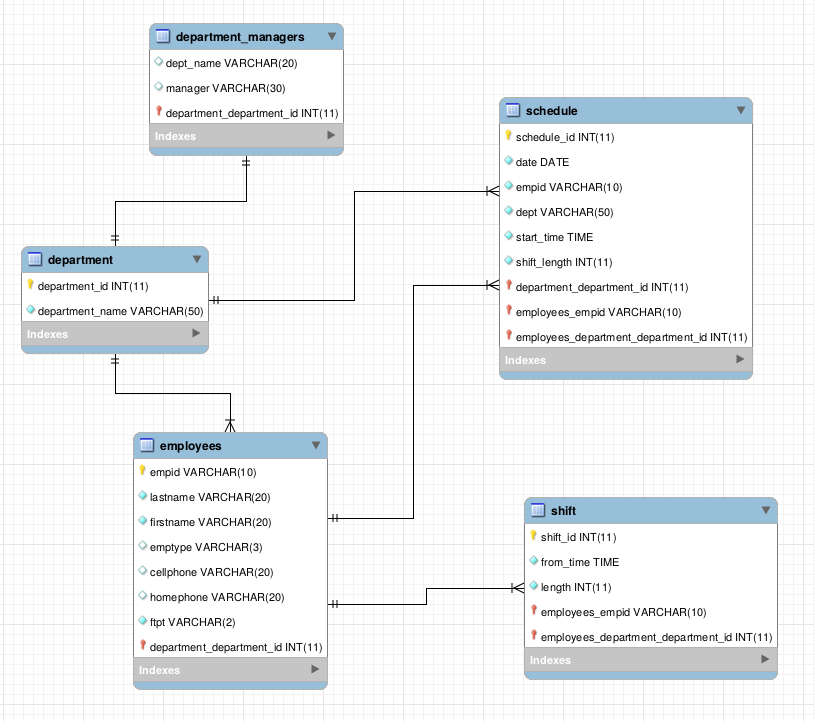
\includegraphics{1.png}
\caption{}
\end{figure}

    \subsection*{SQL Query}\label{sql-query}

\textit{php demo site:
\href{http://cs431project-jxy225.herokuapp.com/}{click here}}

\textit{(source code attached in the submission)}

    \paragraph{1. Show tables}\label{show-tables}

    \begin{Verbatim}[commandchars=\\\{\}]
{\color{incolor}In [{\color{incolor}62}]:} \PY{n}{query} \PY{o}{=} \PY{l+s+s1}{\PYZsq{}}\PY{l+s+s1}{show tables;}\PY{l+s+s1}{\PYZsq{}}
         \PY{n}{tables} \PY{o}{=} \PY{n}{pd}\PY{o}{.}\PY{n}{read\PYZus{}sql}\PY{p}{(}\PY{n}{query}\PY{p}{,} \PY{n}{dsl}\PY{o}{.}\PY{n}{db}\PY{p}{)}
         \PY{n+nb}{print}\PY{p}{(}\PY{n}{tables}\PY{o}{.}\PY{n}{to\PYZus{}latex}\PY{p}{(}\PY{p}{)}\PY{p}{)}
\end{Verbatim}

   \begin{tabular}{|l|l|}
   	\toprule
   	{} & Tables \\
   	\midrule
   	0 &                       department \\
   	1 &              department\_managers \\
   	2 &                        employees \\
   	3 &                         schedule \\
   	4 &                            shift \\
   	\bottomrule
   \end{tabular}

    \paragraph{2. Describe tables}\label{describe-tables}

    \begin{Verbatim}[commandchars=\\\{\}]
{\color{incolor}In [{\color{incolor}55}]:} \PY{k}{for} \PY{n}{table} \PY{o+ow}{in} \PY{n}{tables}\PY{o}{.}\PY{n}{values}\PY{p}{:}
             \PY{n}{query} \PY{o}{=} \PY{l+s+s1}{\PYZsq{}}\PY{l+s+s1}{describe }\PY{l+s+si}{\PYZob{}\PYZcb{}}\PY{l+s+s1}{;}\PY{l+s+s1}{\PYZsq{}}\PY{o}{.}\PY{n}{format}\PY{p}{(}\PY{n}{table}\PY{p}{[}\PY{l+m+mi}{0}\PY{p}{]}\PY{p}{)}
             \PY{n}{df} \PY{o}{=} \PY{n}{pd}\PY{o}{.}\PY{n}{read\PYZus{}sql}\PY{p}{(}\PY{n}{query}\PY{p}{,} \PY{n}{dsl}\PY{o}{.}\PY{n}{db}\PY{p}{)}
             \PY{n+nb}{print}\PY{p}{(}\PY{n}{df}\PY{p}{)}
             \PY{n+nb}{print}\PY{p}{(}\PY{l+s+s1}{\PYZsq{}}\PY{l+s+se}{\PYZbs{}n}\PY{l+s+s1}{\PYZsq{}}\PY{p}{)}
\end{Verbatim}

    \begin{Verbatim}[commandchars=\\\{\}]
             Field         Type Null  Key Default           Extra
0    department\_id      int(11)   NO  PRI    None  auto\_increment
1  department\_name  varchar(50)   NO         None                


       Field         Type Null Key Default Extra
0  dept\_name  varchar(20)  YES        None      
1    manager  varchar(30)  YES        None      


       Field         Type Null  Key Default Extra
0      empid  varchar(10)   NO  PRI    None      
1   lastname  varchar(20)   NO         None      
2  firstname  varchar(20)   NO         None      
3    emptype   varchar(3)  YES         None      
4  cellphone  varchar(20)  YES         None      
5  homephone  varchar(20)  YES         None      
6       ftpt   varchar(2)   NO         None      


          Field         Type Null  Key Default           Extra
0   schedule\_id      int(11)   NO  PRI    None  auto\_increment
1          date         date   NO         None                
2         empid  varchar(10)   NO         None                
3          dept  varchar(50)   NO         None                
4    start\_time         time   NO         None                
5  shift\_length      int(11)   NO         None                


       Field     Type Null  Key Default           Extra
0   shift\_id  int(11)   NO  PRI    None  auto\_increment
1  from\_time     time   NO         None                
2     length  int(11)   NO         None                



    \end{Verbatim}
    
    

    \paragraph{\texorpdfstring{3. Find out the need of employees of certain
type in certain department during certain period \emph{(eg: EMERGENCY,
RN, from 2018-10-03 to
2018-10-11)}}{3. Find out the need of employees of certain type in certain department during certain period (eg: EMERGENCY, RN, from 2018-10-03 to 2018-10-11)}}\label{find-out-the-need-of-employees-of-certain-type-in-certain-department-during-certain-period-eg-emergency-rn-from-2018-10-03-to-2018-10-11}



    \begin{Verbatim}[commandchars=\\\{\}]
{\color{incolor}In [{\color{incolor}91}]:} \PY{n}{query} \PY{o}{=} \PY{l+s+s1}{\PYZsq{}\PYZsq{}\PYZsq{}}
         \PY{l+s+s1}{    SELECT s.dept AS Department,}
         \PY{l+s+s1}{        s.empid AS EmployeeID,}
         \PY{l+s+s1}{        s.date AS Date,}
         \PY{l+s+s1}{        date\PYZus{}format(s.start\PYZus{}time, }\PY{l+s+s1}{\PYZsq{}}\PY{l+s+s1}{\PYZpc{}}\PY{l+s+s1}{I}\PY{l+s+s1}{\PYZpc{}}\PY{l+s+s1}{p}\PY{l+s+s1}{\PYZsq{}}\PY{l+s+s1}{) AS ShiftStartTime,}
         \PY{l+s+s1}{        e.emptype AS EmployeeType}
         \PY{l+s+s1}{                FROM schedule as s, department as d, employees as e}
         \PY{l+s+s1}{                WHERE s.dept=d.department\PYZus{}name}
         \PY{l+s+s1}{                      AND s.empid = e.empid}
         \PY{l+s+s1}{                      AND s.date \PYZgt{}= }\PY{l+s+s1}{\PYZsq{}}\PY{l+s+s1}{2018\PYZhy{}10\PYZhy{}03}\PY{l+s+s1}{\PYZsq{}}
         \PY{l+s+s1}{                      AND s.date \PYZlt{}= }\PY{l+s+s1}{\PYZsq{}}\PY{l+s+s1}{2019\PYZhy{}10\PYZhy{}11}\PY{l+s+s1}{\PYZsq{}}
         \PY{l+s+s1}{                      AND s.dept = }\PY{l+s+s1}{\PYZsq{}}\PY{l+s+s1}{EMERGENCY}\PY{l+s+s1}{\PYZsq{}}
         \PY{l+s+s1}{                      AND e.emptype = }\PY{l+s+s1}{\PYZsq{}}\PY{l+s+s1}{RN}\PY{l+s+s1}{\PYZsq{}}
         \PY{l+s+s1}{                ORDER BY d.department\PYZus{}id, s.date;}
         \PY{l+s+s1}{        }\PY{l+s+s1}{\PYZsq{}\PYZsq{}\PYZsq{}}
         \PY{n}{tables} \PY{o}{=} \PY{n}{pd}\PY{o}{.}\PY{n}{read\PYZus{}sql}\PY{p}{(}\PY{n}{query}\PY{p}{,} \PY{n}{dsl}\PY{o}{.}\PY{n}{db}\PY{p}{)}
         \PY{n+nb}{print}\PY{p}{(}\PY{n}{tables}\PY{o}{.}\PY{n}{to\PYZus{}latex}\PY{p}{(}\PY{p}{)}\PY{p}{)}
\end{Verbatim}



\begin{tabular}{|l|l|l|l|l|l|}
	\toprule
	{} & Department & EmployeeID &        Date & ShiftStartTime & EmployeeType \\
	\midrule
	0 &  EMERGENCY &     940824 &  2018-10-03 &           11PM &           RN \\
	1 &  EMERGENCY &     854480 &  2018-10-04 &           03PM &           RN \\
	2 &  EMERGENCY &     860127 &  2018-10-05 &           07AM &           RN \\
	3 &  EMERGENCY &     945540 &  2018-10-07 &           07AM &           RN \\
	4 &  EMERGENCY &     921331 &  2018-10-07 &           07PM &           RN \\
	\bottomrule
\end{tabular}



    \paragraph{\texorpdfstring{4. Find out whether certain employee has been
scheduled on a certain date \emph{(eg: Remona Locke on
2018-10-03)}}{4. Find out whether certain employee has been scheduled on a certain date (eg: Remona Locke on 2018-10-03)}}\label{find-out-whether-certain-employee-has-been-scheduled-on-a-certain-date-eg-remona-locke-on-2018-10-03}

    \begin{Verbatim}[commandchars=\\\{\}]
{\color{incolor}In [{\color{incolor}92}]:} \PY{n}{query} \PY{o}{=} \PY{l+s+s1}{\PYZsq{}\PYZsq{}\PYZsq{}}
         \PY{l+s+s1}{    SELECT s.schedule\PYZus{}id AS ScheduleID,}
         \PY{l+s+s1}{                            s.empid AS EmployeeID,}
         \PY{l+s+s1}{                            concat(e.firstname, }\PY{l+s+s1}{\PYZsq{}}\PY{l+s+s1}{ }\PY{l+s+s1}{\PYZsq{}}\PY{l+s+s1}{, e.lastname) AS Fullname,}
         \PY{l+s+s1}{                            s.dept AS Department,}
         \PY{l+s+s1}{                            s.date AS Date,}
         \PY{l+s+s1}{                            date\PYZus{}format(s.start\PYZus{}time, }\PY{l+s+s1}{\PYZsq{}}\PY{l+s+s1}{\PYZpc{}}\PY{l+s+s1}{I}\PY{l+s+s1}{\PYZpc{}}\PY{l+s+s1}{p}\PY{l+s+s1}{\PYZsq{}}\PY{l+s+s1}{) AS ShiftStartTime,}
         \PY{l+s+s1}{                            s.shift\PYZus{}length AS ShiftLength}
         \PY{l+s+s1}{                    FROM employees as e, schedule as s}
         \PY{l+s+s1}{                    WHERE s.empid = e.empid}
         \PY{l+s+s1}{                      AND e.firstname = }\PY{l+s+s1}{\PYZsq{}}\PY{l+s+s1}{Remona}\PY{l+s+s1}{\PYZsq{}}
         \PY{l+s+s1}{                      AND e.lastname = }\PY{l+s+s1}{\PYZsq{}}\PY{l+s+s1}{Locke}\PY{l+s+s1}{\PYZsq{}}
         \PY{l+s+s1}{                      AND s.date = }\PY{l+s+s1}{\PYZsq{}}\PY{l+s+s1}{2018\PYZhy{}10\PYZhy{}03}\PY{l+s+s1}{\PYZsq{}}
         \PY{l+s+s1}{        }\PY{l+s+s1}{\PYZsq{}\PYZsq{}\PYZsq{}}
         \PY{n}{tables} \PY{o}{=} \PY{n}{pd}\PY{o}{.}\PY{n}{read\PYZus{}sql}\PY{p}{(}\PY{n}{query}\PY{p}{,} \PY{n}{dsl}\PY{o}{.}\PY{n}{db}\PY{p}{)}
         \PY{n+nb}{print}\PY{p}{(}\PY{n}{tables}\PY{o}{.}\PY{n}{to\PYZus{}latex}\PY{p}{(}\PY{p}{)}\PY{p}{)}
\end{Verbatim}

    \begin{tabular}{|l|r|l|l|l|l|l|r|}
   	\toprule
   	{} &  ScheduleID & EmployeeID &      Fullname & Department &        Date & ShiftStartTime &  ShiftLength \\
   	\bottomrule
   \end{tabular}
   

    \paragraph{5. If not, then this employee is open for
schedule}\label{if-not-then-this-employee-is-open-for-schedule}

    \begin{Verbatim}[commandchars=\\\{\}]
{\color{incolor}In [{\color{incolor}95}]:} \PY{n}{query} \PY{o}{=} \PY{l+s+s1}{\PYZsq{}\PYZsq{}\PYZsq{}}
         \PY{l+s+s1}{    INSERT INTO schedule (date, empid, dept, start\PYZus{}time, shift\PYZus{}length) VALUES}
         \PY{l+s+s1}{                      (}\PY{l+s+s1}{\PYZsq{}}\PY{l+s+s1}{2018\PYZhy{}10\PYZhy{}03}\PY{l+s+s1}{\PYZsq{}}\PY{l+s+s1}{,}
         \PY{l+s+s1}{                       (SELECT empid FROM employees WHERE firstname=}\PY{l+s+s1}{\PYZsq{}}\PY{l+s+s1}{Remona}\PY{l+s+s1}{\PYZsq{}}\PY{l+s+s1}{ AND lastname=}\PY{l+s+s1}{\PYZsq{}}\PY{l+s+s1}{Locke}\PY{l+s+s1}{\PYZsq{}}\PY{l+s+s1}{),}
         \PY{l+s+s1}{                       }\PY{l+s+s1}{\PYZsq{}}\PY{l+s+s1}{EMERGENCY}\PY{l+s+s1}{\PYZsq{}}\PY{l+s+s1}{,}
         \PY{l+s+s1}{                       }\PY{l+s+s1}{\PYZsq{}}\PY{l+s+s1}{12:00:00}\PY{l+s+s1}{\PYZsq{}}\PY{l+s+s1}{,}
         \PY{l+s+s1}{                        8)}
         \PY{l+s+s1}{\PYZsq{}\PYZsq{}\PYZsq{}}
         \PY{n}{dsl}\PY{o}{.}\PY{n}{c}\PY{o}{.}\PY{n}{execute}\PY{p}{(}\PY{n}{query}\PY{p}{)}
\end{Verbatim}

\begin{Verbatim}[commandchars=\\\{\}]
{\color{outcolor}Out[{\color{outcolor}95}]:} 1
\end{Verbatim}
            
    \paragraph{6. Check the schedule}\label{check-the-schedule}

    \begin{Verbatim}[commandchars=\\\{\}]
{\color{incolor}In [{\color{incolor}96}]:} \PY{n}{query} \PY{o}{=} \PY{l+s+s1}{\PYZsq{}\PYZsq{}\PYZsq{}}
         \PY{l+s+s1}{    SELECT s.schedule\PYZus{}id AS ScheduleID,}
         \PY{l+s+s1}{                            s.empid AS EmployeeID,}
         \PY{l+s+s1}{                            concat(e.firstname, }\PY{l+s+s1}{\PYZsq{}}\PY{l+s+s1}{ }\PY{l+s+s1}{\PYZsq{}}\PY{l+s+s1}{, e.lastname) AS Fullname,}
         \PY{l+s+s1}{                            s.dept AS Department,}
         \PY{l+s+s1}{                            s.date AS Date,}
         \PY{l+s+s1}{                            date\PYZus{}format(s.start\PYZus{}time, }\PY{l+s+s1}{\PYZsq{}}\PY{l+s+s1}{\PYZpc{}}\PY{l+s+s1}{I}\PY{l+s+s1}{\PYZpc{}}\PY{l+s+s1}{p}\PY{l+s+s1}{\PYZsq{}}\PY{l+s+s1}{) AS ShiftStartTime,}
         \PY{l+s+s1}{                            s.shift\PYZus{}length AS ShiftLength}
         \PY{l+s+s1}{                    FROM employees as e, schedule as s}
         \PY{l+s+s1}{                    WHERE s.empid = e.empid}
         \PY{l+s+s1}{                      AND e.firstname = }\PY{l+s+s1}{\PYZsq{}}\PY{l+s+s1}{Remona}\PY{l+s+s1}{\PYZsq{}}
         \PY{l+s+s1}{                      AND e.lastname = }\PY{l+s+s1}{\PYZsq{}}\PY{l+s+s1}{Locke}\PY{l+s+s1}{\PYZsq{}}
         \PY{l+s+s1}{                      AND s.date = }\PY{l+s+s1}{\PYZsq{}}\PY{l+s+s1}{2018\PYZhy{}10\PYZhy{}03}\PY{l+s+s1}{\PYZsq{}}
         \PY{l+s+s1}{        }\PY{l+s+s1}{\PYZsq{}\PYZsq{}\PYZsq{}}
         \PY{n}{tables} \PY{o}{=} \PY{n}{pd}\PY{o}{.}\PY{n}{read\PYZus{}sql}\PY{p}{(}\PY{n}{query}\PY{p}{,} \PY{n}{dsl}\PY{o}{.}\PY{n}{db}\PY{p}{)}
         \PY{n+nb}{print}\PY{p}{(}\PY{n}{tables}\PY{o}{.}\PY{n}{to\PYZus{}latex}\PY{p}{(}\PY{p}{)}\PY{p}{)}
\end{Verbatim}

    \begin{tabular}{|l|r|l|l|l|l|l|r|}
    	\toprule
    	{} &  ScheduleID & EmployeeID &      Fullname & Department &        Date & ShiftStartTime &  ShiftLength \\
    	\midrule
    	0 &        4371 &     854480 &  Remona Locke &  EMERGENCY &  2018-10-03 &           12PM &            8 \\
    	\bottomrule
    \end{tabular}
    

    \paragraph{7. Unschedule}\label{unschedule}

    \begin{Verbatim}[commandchars=\\\{\}]
{\color{incolor}In [{\color{incolor}107}]:} \PY{n}{query} \PY{o}{=} \PY{l+s+s1}{\PYZsq{}\PYZsq{}\PYZsq{}}
          \PY{l+s+s1}{    SELECT s.schedule\PYZus{}id}
          \PY{l+s+s1}{         FROM employees as e, schedule as s}
          \PY{l+s+s1}{         WHERE s.empid = e.empid}
          \PY{l+s+s1}{         AND e.firstname = }\PY{l+s+s1}{\PYZsq{}}\PY{l+s+s1}{Remona}\PY{l+s+s1}{\PYZsq{}}
          \PY{l+s+s1}{         AND e.lastname = }\PY{l+s+s1}{\PYZsq{}}\PY{l+s+s1}{Locke}\PY{l+s+s1}{\PYZsq{}}
          \PY{l+s+s1}{         AND s.date = }\PY{l+s+s1}{\PYZsq{}}\PY{l+s+s1}{2018\PYZhy{}10\PYZhy{}03}\PY{l+s+s1}{\PYZsq{}}
          \PY{l+s+s1}{        }\PY{l+s+s1}{\PYZsq{}\PYZsq{}\PYZsq{}}
          \PY{n}{dsl}\PY{o}{.}\PY{n}{c}\PY{o}{.}\PY{n}{execute}\PY{p}{(}\PY{n}{query}\PY{p}{)}
          \PY{n}{schedule\PYZus{}id}  \PY{o}{=} \PY{n}{dsl}\PY{o}{.}\PY{n}{c}\PY{o}{.}\PY{n}{fetchall}\PY{p}{(}\PY{p}{)}\PY{p}{[}\PY{l+m+mi}{0}\PY{p}{]}\PY{p}{[}\PY{l+m+mi}{0}\PY{p}{]}
          \PY{n}{query} \PY{o}{=} \PY{l+s+s1}{\PYZsq{}\PYZsq{}\PYZsq{}}
          \PY{l+s+s1}{    DELETE FROM schedule WHERE schedule\PYZus{}id=}\PY{l+s+si}{\PYZob{}\PYZcb{}}
          \PY{l+s+s1}{    }\PY{l+s+s1}{\PYZsq{}\PYZsq{}\PYZsq{}}\PY{o}{.}\PY{n}{format}\PY{p}{(}\PY{n}{schedule\PYZus{}id}\PY{p}{)}
          \PY{n}{dsl}\PY{o}{.}\PY{n}{c}\PY{o}{.}\PY{n}{execute}\PY{p}{(}\PY{n}{query}\PY{p}{)}
\end{Verbatim}

\begin{Verbatim}[commandchars=\\\{\}]
{\color{outcolor}Out[{\color{outcolor}107}]:} 1
\end{Verbatim}
            
    \paragraph{8. Check the employee has been
unscheduled}\label{check-the-employee-has-been-unscheduled}

    \begin{Verbatim}[commandchars=\\\{\}]
{\color{incolor}In [{\color{incolor}111}]:} \PY{n}{query} \PY{o}{=} \PY{l+s+s1}{\PYZsq{}\PYZsq{}\PYZsq{}}
          \PY{l+s+s1}{    SELECT s.schedule\PYZus{}id AS ScheduleID,}
          \PY{l+s+s1}{                            s.empid AS EmployeeID,}
          \PY{l+s+s1}{                            concat(e.firstname, }\PY{l+s+s1}{\PYZsq{}}\PY{l+s+s1}{ }\PY{l+s+s1}{\PYZsq{}}\PY{l+s+s1}{, e.lastname) AS Fullname,}
          \PY{l+s+s1}{                            s.dept AS Department,}
          \PY{l+s+s1}{                            s.date AS Date,}
          \PY{l+s+s1}{                            date\PYZus{}format(s.start\PYZus{}time, }\PY{l+s+s1}{\PYZsq{}}\PY{l+s+s1}{\PYZpc{}}\PY{l+s+s1}{I}\PY{l+s+s1}{\PYZpc{}}\PY{l+s+s1}{p}\PY{l+s+s1}{\PYZsq{}}\PY{l+s+s1}{) AS ShiftStartTime,}
          \PY{l+s+s1}{                            s.shift\PYZus{}length AS ShiftLength}
          \PY{l+s+s1}{                    FROM employees as e, schedule as s}
          \PY{l+s+s1}{                    WHERE s.empid = e.empid}
          \PY{l+s+s1}{                      AND e.firstname = }\PY{l+s+s1}{\PYZsq{}}\PY{l+s+s1}{Remona}\PY{l+s+s1}{\PYZsq{}}
          \PY{l+s+s1}{                      AND e.lastname = }\PY{l+s+s1}{\PYZsq{}}\PY{l+s+s1}{Locke}\PY{l+s+s1}{\PYZsq{}}
          \PY{l+s+s1}{                      AND s.date = }\PY{l+s+s1}{\PYZsq{}}\PY{l+s+s1}{2018\PYZhy{}10\PYZhy{}03}\PY{l+s+s1}{\PYZsq{}}
          \PY{l+s+s1}{        }\PY{l+s+s1}{\PYZsq{}\PYZsq{}\PYZsq{}}
          \PY{n}{tables} \PY{o}{=} \PY{n}{pd}\PY{o}{.}\PY{n}{read\PYZus{}sql}\PY{p}{(}\PY{n}{query}\PY{p}{,} \PY{n}{dsl}\PY{o}{.}\PY{n}{db}\PY{p}{)}
          \PY{n+nb}{print}\PY{p}{(}\PY{n}{tables}\PY{o}{.}\PY{n}{to\PYZus{}latex}\PY{p}{(}\PY{p}{)}\PY{p}{)}
\end{Verbatim}

   \begin{tabular}{|l|r|l|l|l|l|l|r|}
   	\toprule
   	{} &  ScheduleID & EmployeeID &      Fullname & Department &        Date & ShiftStartTime &  ShiftLength \\
   	\bottomrule
   \end{tabular}
   


    % Add a bibliography block to the postdoc
    
    
    
    \end{document}
